%!TEX program = xelatex
\documentclass[dvipsnames, svgnames,a4paper,11pt]{article}
% ----------------------------------------------------
%   吉林大学通信工程学院信号与系统实验报告
%   原作者:Huanyu Shi,2019级
%     知乎:https://www.zhihu.com/people/za-ran-zhu-fu-liu-xing
%     Github:https://github.com/huanyushi/SYSU-SPA-Labreport-Template
%   在原基础上魔改了一些,更加贴近吉林大学实验格式。
% ----------------------------------------------------

% ----------------------------------------------------- 
%	加边框的命令
%	参考:https://tex.stackexchange.com/questions/531559/how-to-add-the-page-border-for-first-two-pages-in-latex
\usepackage{tikz}
\usetikzlibrary{calc}
\usepackage{eso-pic}
\AddToShipoutPictureBG{%
\begin{tikzpicture}[overlay,remember picture]
\draw[line width=0.6pt] % 边框粗细
    ($ (current page.north west) + (0.6cm,-0.6cm) $)
    rectangle
    ($ (current page.south east) + (-0.6cm,0.6cm) $); % 边框位置
\end{tikzpicture}}


\usepackage{xcolor}
\definecolor{c1}{HTML}{2752C9} % 目录颜色
\definecolor{c2}{RGB}{190,20,83} % 引用颜色

\usepackage{ctex}
\usepackage[top=28mm,bottom=28mm,left=15mm,right=15mm]{geometry}
\usepackage{hyperref} 
\hypersetup{
	colorlinks,
	linktoc = section, % 超链接位置,选项有section, page, all
	linkcolor = c1, % linkcolor 目录颜色
	citecolor = c1  % citecolor 引用颜色
}
\usepackage{amsmath,enumerate,multirow,float}
\usepackage{tabularx}
\usepackage{tabu}
\usepackage{subfig}
\usepackage{fancyhdr}
\usepackage{graphicx}
\usepackage{wrapfig}  
\usepackage{physics}
\usepackage{appendix}
\usepackage{amsfonts}

%
\usepackage{tcolorbox}
\tcbuselibrary{skins,breakable}
\newtcolorbox{tbox}[2][]{
    colframe=black!70!,
    breakable,
    enhanced,
	boxrule =0.5pt,
    title = {#2},
    fonttitle = \large\kaishu\bfseries,
	drop fuzzy shadow,
    #1
}
\newtcolorbox[auto counter,number within=section]{question}[1][]{
  top=2pt,bottom=2pt,arc=1mm,
  boxrule=0.5pt,
%   frame hidden,
  breakable,
  enhanced, %跨页后不会显示下边框
  coltitle=c1!80!gray,
  colframe=c1,
  colback=c1!3!white,
  drop fuzzy shadow,
  title={思考题~\thetcbcounter:\quad},
  fonttitle=\bfseries,
  attach title to upper,
  #1
}

% ---------------------------------------------------------------------
%	利用cleveref改变引用格式,\cref是引用命令
\usepackage{cleveref}
\crefformat{figure}{#2{\textcolor{c2}{图 #1}}#3} % 图片的引用格式
\crefformat{equation}{#2{(\textcolor{c2}{#1})}#3} % 公式的引用格式
\crefformat{table}{#2{\textcolor{c2}{表 #1}}#3} % 表格的引用格式


% ---------------------------------------------------------------------
%	页眉页脚设置
\fancypagestyle{plain}{\pagestyle{fancy}}
\pagestyle{fancy}
\lhead{\kaishu 吉林大学通信工程学院} % 左边页眉,学院 + 课程
\rhead{\kaishu 信号与系统实验报告} % 右边页眉,实验报告标题
\cfoot{\thepage} % 页脚,中间添加页码


% ---------------------------------------------------------------------
%	对目录、章节标题的设置
\renewcommand{\contentsname}{\centerline{\huge 目录}}
\usepackage{titlesec}
\usepackage{titletoc}
% \titleformat{章节}[形状]{格式}{标题序号}{序号与标题间距}{标题前命令}[标题后命令]
\titleformat{\section}{\centering\LARGE\songti}{}{1em}{}

% ---------------------------------------------------------------------
%   listing代码环境设置
\usepackage{listings}
\lstloadlanguages{python}
\lstdefinestyle{pythonstyle}{
backgroundcolor=\color{gray!5},
language=python,
frameround=tftt,
frame=shadowbox, 
keepspaces=true,
breaklines,
columns=spaceflexible,                   
basicstyle=\ttfamily\small, % 基本文本设置,字体为teletype,大小为scriptsize
keywordstyle=[1]\color{c1}\bfseries, 
keywordstyle=[2]\color{Red!70!black},   
stringstyle=\color{Purple},       
showstringspaces=false,
commentstyle=\ttfamily\scriptsize\color{green!40!black},%注释文本设置,字体为sf,大小为smaller
tabsize=2,
morekeywords={as},
morekeywords=[2]{np, plt, sp},
numbers=left, % 代码行数
numberstyle=\it\tiny\color{gray}, % 代码行数的数字字体设置
stepnumber=1,
rulesepcolor=\color{gray!30!white}
}




% ---------------------------------------------------------------------
%	其他设置
\def\degree{${}^{\circ}$} % 角度
\graphicspath{{./images/}} % 插入图片的相对路径
\allowdisplaybreaks[4]  %允许公式跨页


%---------------------------------------------------------------------------%
%->> User defined commands
%---------------------------------------------------------------------------%
\RequirePackage{mathrsfs}% script style math symbols % 导入模板的相关设置
\usepackage{lipsum}
\usepackage{amsmath}


%---------------------------------------------------------------------
%	正文
%---------------------------------------------------------------------

\begin{document}

\begin{table}
  \raggedleft
	\renewcommand\arraystretch{1.7}
	\begin{tabular}{|c|p{4em}|}
	\hline
	成绩 &  \\
	\hline
	教师签字 &   \\
	\hline
	\end{tabular}
\end{table}

\begin{center}
	{\kaishu \LARGE   \quad  \quad 通  \quad 信  \quad 工  \quad 程  \quad 学  \quad 院 }
  \newline
  \newline
  \newline
  \newline
  \newline
  {\kaishu \Huge 实 \quad  \quad  \quad 验  \quad  \quad  \quad 报 \quad  \quad  \quad 告}
  \newline
  \newline
  \newline
  \newline
  \newline
  {\songti \Huge  ( \quad  信  \quad 号  \quad 与  \quad 系  \quad 统 \quad)}
  \newline
  \newline
  \newline
  \newline
  \newline
  {\songti  \LARGE 实验题目:非正弦周期信号的分解与合成  \quad  \quad \quad}
\end{center}



\begin{table}[b]
	\renewcommand\arraystretch{1.7}
	\begin{tabularx}{\textwidth}{|X|X|X|X|}
	\hline
	专业:& 通信工程 &年级:& 2022级\\
	\hline
	姓名:& 苏睿杰  & 学号:& 20220826\\
	\hline
	实验时间:& 2023年11月24日 & 班级:& 42 \\
	\hline
	\end{tabularx}
\end{table}


%\clearpage
%\tableofcontents

\clearpage
\setcounter{section}{0}
\section{实验十六 \quad 非正弦周期信号的分解与合成}
\subsection*{一、实验目的}
\begin{enumerate}
  \item 用实验方法观测非正弦周期信号的分解,并与其傅利叶级数各项的频率与系数作比较。 
  \item 观测基波和其谐波的合成。
\end{enumerate}

\subsection*{二、仪器设备}
\begin{enumerate}
  \item 实验箱一台。
  \item 数字示波器。
\end{enumerate}

\subsection*{三、原理说明}
任何信号都是由各种不同频率、幅度和初相的正弦波叠加而成的。由非正弦周期信号傅里叶级数展开式可知,各次谐波为基波频率的整数倍。而第一个非周期信号包含了从零到无穷大的所有频率成分,其幅度将随谐波次数的增高而减小,直至无穷小,将被测信号加到分别调谐于其基波和各次谐波频率的电路上。从每一带通滤器的输出端可以用示波器观察到相应频率的正弦波。本实验所用的被测信号是选用 $50Hz$ 的方波、矩形波、三角波、全波和半波等。

\subsection*{四、理论值的计算}
\begin{figure}[htbp]
  \centering
  \begin{minipage}[t]{0.48\textwidth}
  \centering
  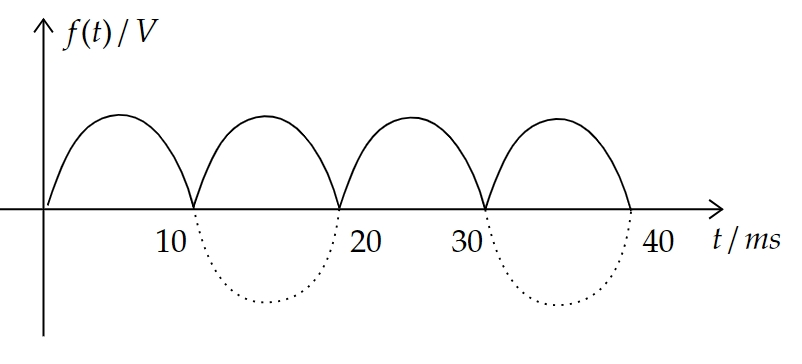
\includegraphics[width=9cm]{1.png}
  \caption{全波整流信号}
  \end{minipage}
  \begin{minipage}[t]{0.48\textwidth}
  \centering
  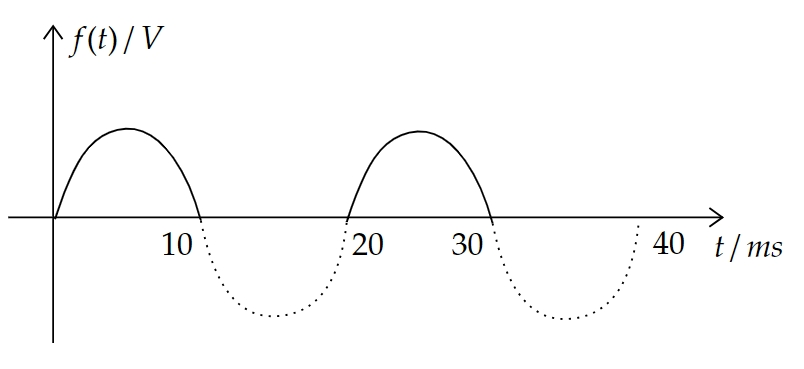
\includegraphics[width=9cm]{2.png}
  \caption{半波整流信号}
  \end{minipage}
\end{figure}

\begin{enumerate}
  \item 基频为50Hz的方波的谐波型傅里叶级数
    
    将方波信号的傅里叶级数展开:

    \begin{equation*}
      f(t) = a_0 + \sum_{n = 1}^{\infty} \left [ a_n \cos (n\omega t) + b_n \sin (n\omega t) \right ]
    \end{equation*}

    利用公式可算得

    \begin{align*}
      & a_0 = \dfrac{1}{T}\int_{0}^{T}f(t)dt = 0 \\
      & a_n = \dfrac{2}{T}\int_{0}^{T}f(t)\cos (n\omega t)dt = 0 \\
      & b_n = \dfrac{2}{T}\int_{0}^{T}f(t)\sin (n\omega t)dt = \dfrac{4}{n\pi}\sin^2 (\dfrac{n\pi}{2})
    \end{align*}
      
    又由于

    \begin{align*}
      & A_n = \sqrt{a_n^2 + b_n^2} = \dfrac{4}{n\pi}\sin^2 (\dfrac{n\pi}{2})\\
      & \varphi_n = -\arctan (\dfrac{b_n}{a_n}) = -\dfrac{\pi}{2}
    \end{align*}
      
    最后可得到

    \begin{equation*}
      f(t) = \sum_{i = 1}^{\infty} \dfrac{4}{n\pi}\sin^2 (\dfrac{n\pi}{2}) \cos(n\omega t -\dfrac{\pi}{2})
    \end{equation*}

  \item 基频为50Hz的三角波的谐波型傅里叶级数
  
  将三角波信号的傅里叶级数展开:

  \begin{equation*}
    f(t) = a_0 + \sum_{n = 1}^{\infty} \left [ a_n \cos (n\omega t) + b_n \sin (n\omega t) \right ]
  \end{equation*}

  利用公式可算得

  \begin{align*}
    & a_0 = \dfrac{1}{T}\int_{0}^{T}f(t)dt = 0 \\
    & a_n = \dfrac{2}{T}\int_{0}^{T}f(t)\cos (n\omega t)dt = 0 \\
    & b_n = \dfrac{2}{T}\int_{0}^{T}f(t)\sin (n\omega t)dt = \dfrac{8}{(n\pi)^2}\sin (\dfrac{n\pi}{2})
  \end{align*}
    
  又由于

  \begin{align*}
    & A_n = \sqrt{a_n^2 + b_n^2} = \dfrac{8}{(n\pi)^2}\sin (\dfrac{n\pi}{2})\\
    & \varphi_n = -\arctan (\dfrac{b_n}{a_n}) = -\dfrac{\pi}{2}
  \end{align*}
    
  最后可得到

  \begin{equation*}
    f(t) = \sum_{i = 1}^{\infty} \dfrac{8}{(n\pi)^2}\sin (\dfrac{n\pi}{2})\cos(n\omega t - \dfrac{\pi}{2}) 
  \end{equation*}


  \item 基频为50Hz的锯齿波的谐波型傅里叶级数

  将锯齿波信号的傅里叶级数展开:

  \begin{equation*}
    f(t) = a_0 + \sum_{n = 1}^{\infty} \left [ a_n \cos (n\omega t) + b_n \sin (n\omega t) \right ]
  \end{equation*}

  利用公式可算得

  \begin{align*}
    & a_0 = \dfrac{1}{T}\int_{0}^{T}f(t)dt = \dfrac{1}{2} \\
    & a_n = \dfrac{2}{T}\int_{0}^{T}f(t)\cos (n\omega t)dt = \dfrac{2}{n^2\omega^2 T^2} [1 - \cos(n\omega T)] = 0 \\
    & b_n = \dfrac{2}{T}\int_{0}^{T}f(t)\sin (n\omega t)dt = \dfrac{1}{n\pi}
  \end{align*}
    
  又由于

  \begin{align*}
    & A_n = \sqrt{a_n^2 + b_n^2} = \dfrac{1}{n\pi}\\
    & \varphi_n = -\arctan (\dfrac{b_n}{a_n}) = -\dfrac{\pi}{2}
  \end{align*}
    
  最后可得到

  \begin{equation*}
    f(t) = \dfrac{1}{2} + \sum_{i = 1}^{\infty} \dfrac{4}{n\omega T}\sin (\dfrac{n\omega T}{2}) \cos(n\omega t - \dfrac{n\omega \tau}{2})
  \end{equation*}



\end{enumerate}



\subsection*{五、实验内容及步骤}
\begin{enumerate}
  \item 调节函数信号发生器,使其输出为 $50Hz$ 方波。将其接至该实验模块的输入端,再细调函数信号发生器的输出,使 $50Hz$(基波)的 BPF 模块有最大的输出。然后,将各带通滤波器的输出分别接至示波器和交流亳伏表,观测各次谐波的频率和幅度,并记录之。
  \item 将方波分解所得的基波和三次谐波分量接至加法器的相应输入端,观测加法器的输出波形,并记录所得的波形。
  \item 再将方波的五次谐波分量加到加法器的相应输入端,观测相加后的波形,记录之。
  \item 分别输入 $50Hz$ 的矩形波、三角波、全波和半波信号,并分别观测谐波分量,记录波形的幅值及频率。
  \item 在加法器的输入端接入相应的各谐波分量,进行信号的合成实验,观察频率失真,并记录结果。
\end{enumerate}

\end{document}